\documentclass[aspectratio=169]{../latex_main/tntbeamer}  % you can pass all options of the beamer class, e.g., 'handout' or 'aspectratio=43'
\usepackage{dsfont}
\usepackage{bm}
\usepackage[english]{babel}
\usepackage[T1]{fontenc}
%\usepackage[utf8]{inputenc}
\usepackage{graphicx}
\graphicspath{ {./figures/} }
\usepackage{algorithm}
\usepackage[ruled,vlined,algo2e,linesnumbered]{algorithm2e}
\usepackage{hyperref}
\usepackage{booktabs}
\usepackage{mathtools}

\usepackage{amsmath,amssymb}

\DeclareMathOperator*{\argmax}{arg\,max}
\DeclareMathOperator*{\argmin}{arg\,min}

\usepackage{amsbsy}
\newcommand{\vect}[1]{\bm{#1}}
%\newcommand{\vect}[1]{\boldsymbol{#1}}

\usepackage{pgfplots}
\pgfplotsset{compat=1.16}
\usepackage{tikz}
\usetikzlibrary{trees} 
\usetikzlibrary{shapes.geometric}
\usetikzlibrary{positioning,shapes,shadows,arrows,calc,mindmap}
\usetikzlibrary{positioning,fadings,through}
\usetikzlibrary{decorations.pathreplacing}
\usetikzlibrary{intersections}
\pgfdeclarelayer{background}
\pgfdeclarelayer{foreground}
\pgfsetlayers{background,main,foreground}
\tikzstyle{activity}=[rectangle, draw=black, rounded corners, text centered, text width=8em]
\tikzstyle{data}=[rectangle, draw=black, text centered, text width=8em]
\tikzstyle{myarrow}=[->, thick, draw=black]

% Define the layers to draw the diagram
\pgfdeclarelayer{background}
\pgfdeclarelayer{foreground}
\pgfsetlayers{background,main,foreground}

% Requires XeLaTeX or LuaLaTeX
%\usepackage{unicode-math}

\usepackage{fontspec}
%\setsansfont{Arial}
\setsansfont{RotisSansSerifStd}[ 
Path=../latex_main/fonts/,
Extension = .otf,
UprightFont = *-Regular,  % or *-Light
BoldFont = *-ExtraBold,  % or *-Bold
ItalicFont = *-Italic
]
\setmonofont{Cascadia Mono}[
Scale=0.8
]

% scale factor adapted; mathrm font added (Benjamin Spitschan @TNT, 2021-06-01)
%\setmathfont[Scale=1.05]{Libertinus Math}
%\setmathrm[Scale=1.05]{Libertinus Math}

% other available math fonts are (not exhaustive)
% Latin Modern Math
% XITS Math
% Libertinus Math
% Asana Math
% Fira Math
% TeX Gyre Pagella Math
% TeX Gyre Bonum Math
% TeX Gyre Schola Math
% TeX Gyre Termes Math

% Literature References
\newcommand{\lit}[2]{\href{#2}{\footnotesize\color{black!60}[#1]}}

%%% Beamer Customization
%----------------------------------------------------------------------
% (Don't) Show sections in frame header. Options: 'sections', 'sections light', empty
\setbeamertemplate{headline}{empty}

% Add header logo for normal frames
\setheaderimage{
	% 
\includegraphics[height=\logoheight]{figures/TNT_darkv4.pdf}
	
\includegraphics[height=\logoheight]{../latex_main/figures/luh_logo_rgb_0_80_155.pdf}
	% 
\includegraphics[height=\logoheight]{figures/logo_tntluh.pdf}
}

% Header logo for title page
\settitleheaderimage{
	% 
\includegraphics[height=\logoheight]{figures/TNT_darkv4.pdf}
	
\includegraphics[height=\logoheight]{../latex_main/figures/luh_logo_rgb_0_80_155.pdf}
	% 
\includegraphics[height=\logoheight]{figures/logo_tntluh.pdf}
}

% Title page: tntdefault 
\setbeamertemplate{title page}[tntdefault]  % or luhstyle
% Add optional title image here
%\addtitlepageimagedefault{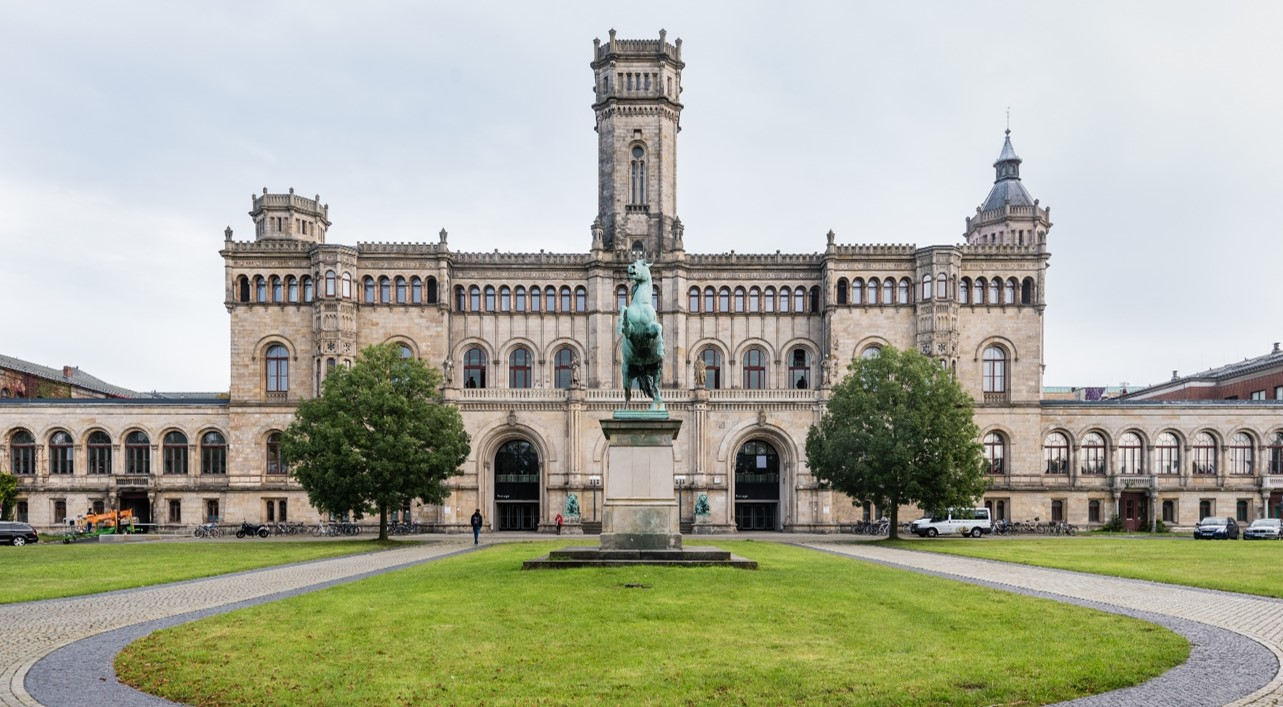
\includegraphics[width=0.65\textwidth]{figures/luh_default_presentation_title_image.jpg}}

% Title page: luhstyle
% \setbeamertemplate{title page}[luhstyle]
% % Add optional title image here
% \addtitlepageimage{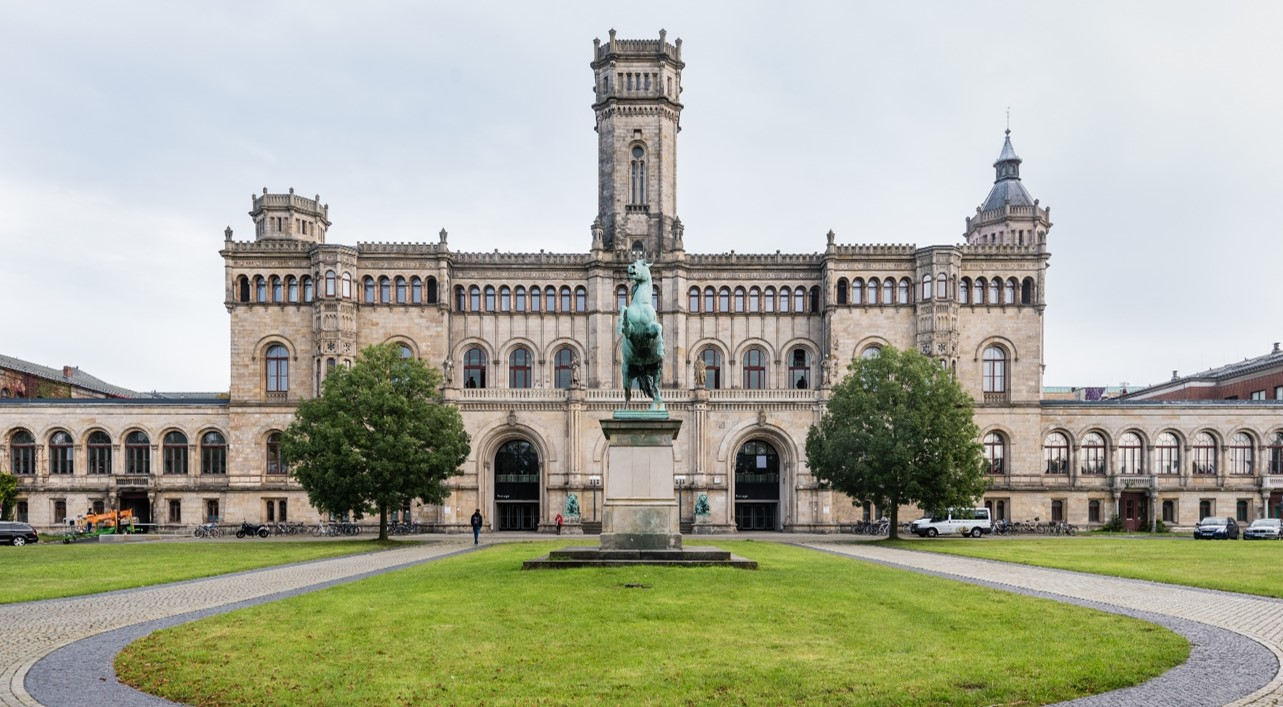
\includegraphics[width=0.75\textwidth]{figures/luh_default_presentation_title_image.jpg}}

\author[Abedjan \& Lindauer]{Ziawasch Abedjan \& Marius Lindauer\\[1em]
	
\includegraphics[height=\logoheight]{../latex_main/figures/luh_logo_rgb_0_80_155.pdf}\qquad
	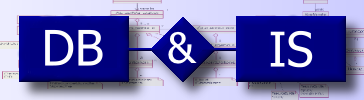
\includegraphics[height=\logoheight]{../latex_main/figures/DBIS_Kurzlogo.png}\qquad

\includegraphics[height=\logoheight]{../latex_main/figures/TNT_darkv4}\qquad

\includegraphics[height=\logoheight]{../latex_main/figures/L3S.jpg}	}
\date{Summer Term 2022; \hspace{0.5em} {
\includegraphics[height=1.5em]{../latex_main/figures/Cc-by-nc-sa_icon.svg.png}}; based on \href{https://ds100.org/fa21/}{[DS100]}
}


%%% Custom Packages
%----------------------------------------------------------------------
% Create dummy content
\usepackage{blindtext}

% Adds a frame with the current page layout. Just call \layout inside of a frame.
\usepackage{layout}


%%% Macros
%\renewcommand{\vec}[1]{\mathbf{#1}}
% \usepackage{bm}
%\let\vecb\bm

\title[Introduction]{DS: Data Cleaning and EDA}
\subtitle{Faithfulness and Missing Values}

\graphicspath{ {./figure/} }
%\institute{}


\begin{document}
	
	\maketitle
	
		\begin{frame}{Key Data Properties to Consider in EDA}
	    \begin{itemize}
	        \item Structure -- the “shape” of a data file
	        \item Granularity -- how fine/coarse is each datum
	        \item Scope -- how (in)complete is the data
	        \item Temporality -- how is the data situated in time
	        \item \textbf{Faithfulness -- how well does the data capture “reality”}
	    \end{itemize}
	\end{frame}
	
	
	\begin{frame}{Faithfulness: Do I trust this data?}
	    \begin{itemize}
	        \item Does my data contain unrealistic or “incorrect” values?
	        \begin{itemize}
	            \item Dates in the future for events in the past
	            \item Locations that don’t exist
	            \item Negative counts
	            \item Misspellings of names
	            \item Large outliers
	        \end{itemize}
	        \item Does my data violate obvious dependencies?
	        \begin{itemize}
	            \item E.g., age and birthday don’t match 
	        \end{itemize}
	        \item Was the data entered by hand?
	        \begin{itemize}
	            \item Spelling errors, fields shifted …
	            \item Did the form require fields or provide default values?
	        \end{itemize}
	        \item Are there obvious signs of data falsification:
	        \begin{itemize}
	            \item Repeated names, fake looking email addresses, repeated use of uncommon names or fields.
	        \end{itemize}
	    \end{itemize}
	\end{frame}
	
	
	
	\begin{frame}{Signs that your data may not be faithful}
	    \begin{itemize}
	        \item Missing Values/Default values?
	        \begin{itemize}
	            \item What do they look like?
	            \begin{itemize}
	                \item “   “, 
	                \item 0, 
	                \item -1, 999, 12345, 
	                \item NaN, Null, 
	                \item 1970, 1900
	            \end{itemize}
	    \end{itemize}
	    \end{itemize}
	\end{frame}
	
	
	
	\begin{frame}{What to do with the Missing Values?}
	    \begin{itemize}
	        \item Drop records with missing values
	        \begin{itemize}
	            \item Probably most common
	            \item Caution: check for biases introduced by dropped values
	            \begin{itemize}
	                \item Missing or corrupt records might be related to something of interest
	            \end{itemize}
	        \end{itemize}
	        \item Imputation: (Inferring missing values)
            \begin{itemize}
                \item Mean Imputation: replace with an average value 
                \begin{itemize}
                    \item Which mean?  Often use closest related subgroup mean.
                \end{itemize}
                \item Hot deck imputation: replace with a random value
                \begin{itemize}
                    \item Choose a random value from the subgroup and use it for the missing value.
                \end{itemize}
                \item Prof. Gonzalez Suggestion: 
                \begin{itemize}
                    \item Drop missing values but check for induced bias (use domain knowledge)
                    \item Directly model missing values during future analysis
                \end{itemize}
            \end{itemize}
            
	    \end{itemize}
	\end{frame}
	
	
	
	\begin{frame}{Signs that your data may not be faithful}
	    \begin{itemize}
	        \item Missing Values or default values
	        \item Truncated data (early excel limits: 65536 Rows, 255 Columns)
	        \begin{itemize}
	            \item Soln: be aware of consequences in analysis ⇒ how did truncation affect sample?
	        \end{itemize}
	        \item Time Zone Inconsistencies
            \begin{itemize}
                \item Soln 1: convert to a common timezone (e.g., UTC) 
                \item Soln 2: convert to the timezone of the location – useful in modeling behavior.
            \end{itemize}
            \item Duplicated Records or Fields
            \begin{itemize}
                \item Soln: identify and eliminate (use primary key) ⇒ implications on sample?
            \end{itemize}
            \item Spelling Errors
            \begin{itemize}
                \item Soln: Apply corrections or drop records not in a dictionary ⇒ implications on sample?
            \end{itemize}
            \item Units not specified or consistent
            \begin{itemize}
                \item Solns: Infer units, check values are in reasonable ranges for data
            \end{itemize}
            \item Others…
	    \end{itemize}
	\end{frame}
\end{document}